\documentclass[a4paper, 12pt]{article}
\usepackage[left=3cm,
            right=3cm,
            top=3cm,
            bottom=3cm,
            bindingoffset=0cm]{geometry}
\usepackage{setspace}
\onehalfspacing

\usepackage[english,russian]{babel}

% FORMATTING
\usepackage{hyperref}

% TYPOGRAPHY
\usepackage{amsmath}
\usepackage{stmaryrd}
% \usepackage{mathspec}
\usepackage{fontspec}
\usepackage{unicode-math}

\setmainfont{Libertinus Serif}
\setsansfont{Libertinus Sans}
\setmathfont{Libertinus Math}

\usepackage[normalem]{ulem}

% LINGUISTICS 
% \usepackage{expex}
% \lingset{aboveglftskip=0ex, belowglpreambleskip=0ex, belowexskip=1ex, aboveexskip=1ex, interpartskip=0ex}
% \gathertags
% \let\expexgla\gla % dumb unicode-math conflict
% \AtBeginDocument{\let\gla\expexgla}

\usepackage{expex}

\usepackage{leipzig}
\newleipzig{cmpr}{cmpr}{Comparative}
\newleipzig{sprl}{sprl}{Superlative}
\newleipzig{indef}{indef}{Indefinite}


% SUBSTITUTION
\usepackage{hyphsubst}
\usepackage{csquotes}
\MakeOuterQuote{"}

% BIBLIOGRAPHY		    
% \usepackage[style=authoryear,url=false,doi=false,isbn=false,eprint=false,date=year]{biblatex}
\usepackage[style=gost-footnote,language=auto,autolang=other,url=false,doi=false,isbn=false,eprint=false,date=year]{biblatex}

\addbibresource{../../ref.bib}

% \usepackage{natbib}
% \renewcommand{\bibsection}{~\\\textbf{References}}
% \bibpunct[: ]{[}{]}{;}{a}{}{,}
% \bibliographystyle{rusnat}

% DRAWING
\usepackage{tikz}
\usepackage{tikz-qtree}
\usetikzlibrary{shapes.geometric}
\usetikzlibrary{trees,arrows}
\usetikzlibrary{positioning}


\begin{document}

% -------------------------- текстиктекстиктекстик -----------------------------
\section{Влияение порядка слов на определенность в русском языке: экспериментальное исследование}
\subsection{Введение}

Известно, что порядок слов в русском языке, как и во многих других, определяется информационной структурой \parencite{slyusar2018nastyketeoriy}: топикальные составляющие тяготеют к более левой позиции в клаузе. В то же время многими исследователями отмечалось, что помимо этого порядок слов в языках без артиклей, в том числе в русском, влияет на интерпретацию ИГ как определенных или неопределенных \parencite[и пр.]{brun2001informationstructurestatus,geist2010baresingularnps}.

В частности, \textcite{geist2010baresingularnps} показывает, что предглагольные голые именные группы, в отличие от постглагольных, не могут быть неопределенными (соответствовать английским ИГ с \textit{a}) (\nextx).

\pex<>
    \a<> На том столе лежит книга. \trailingcitation{`the book' / `a book'}
    \a<> Книга лежит на том столе. \trailingcitation{только `the book'}
\xe

В то же время, согласно Гейст, это ограничение исчезает, когда предгалгольная ИГ несет фразовый акцент (\nextx).

\pex<wo>
    \a<> Метеорит \textsc{упал}\textsubscript{F}. \trailingcitation{только `the meteorite'}
    \a<> \textsc{Метеорит}\textsubscript{F} упал. \trailingcitation{`the meteorite' / `a meteorite'}.
\xe

В то же время обобщение «ИГ может быть неопределенной, только если она фокусно маркирована» неверно: неопределенные ИГ также могут быть контекстно салиентными и, соответственно, не нести фразового акцента (\nextx).

\ex<>
    У кого есть карандаш?\\
    \textsc{У Нины}\textsubscript{F} есть карандаш.
\xe

Гейст заключает, что голые именные группы могут быть неопределенными, только когда не являются топикальными. В то же время остается открытым вопрос, что определяет порядок слов в тетических предложениях, таких как (\getfullref{wo}). Так или иначе, теоретический анализ пресуппозиций, вызываемых порядком слов, невозможен без получения точных данных о том, в каких ситуациях и какие именно пресуппозиции возникают. Из-за высокой вариативности и связи с информационной структурой для этих целей необходимы экспериментальные данные, полученные при контролировании различных переменных.

\subsection{Предыдущие исследования}

Два эксперимента, поставленных Шимиком и Демианом \parencite{simik2020definitenessuniquenessmaximality,simik2021uniquenessmaximalitygerman}, ставили целью подтвердить интуиции исследователей, постулирующих требование на определенность приглагольных именных групп. Объектом обоих экспериментов были предложения с неаккузативным глаголом и без адъюнктов. Оба эксперимента были для сравнения поставлены на одном из славянских языков и немецком.

Первый эксперимент (n\textsubscript{рус} = n\textsubscript{нем} = 48) \parencite{simik2020definitenessuniquenessmaximality} исследовал наличие пресуппозиции уникальности (для ИГ в единственном числе) и максимальности (для ИГ во множественном числе) при восприятии предложений на русском и на немецком. Эксперимент использовал дизайн со скрытыми карточками:

\begin{enumerate}
    \item Участник видит две «перевернутые» карточки — серых прямоугольника — и прослушивает стимул, состоящий из преамбулы и целевого предложения.
    \item Одна из двух карточек «переворачивается» — вместо нее появляется изображение. Участник должен выбрать одну из двух карточек, которая, как ему кажется, лучше (потенциально) описывает ситуацию — открытую или закрытую.
    \item По совершении выбора происходит переход к следующему стимулу. Закрытая карточка не раскрывается.
\end{enumerate}

Русские стимулы варьировались по порядку глагола и субъекта и по положению фокусного акцента — на глаголе или на субъекте, а также по числу. Таким образом каждый стимул имел один из шести вариантов (неприемлемые варианты с порядком слов VS и фокусным акцентом на глаголе в эксперимент не входили) (\nextx). Немецкие стимулы различались наличием определенного артикля.

\pex<>
    \a<> Отцепился \textsc{вагон}.
    \a<> Вагон \textsc{отцепился}.
    \a<> Вагон \textsc{отцепился}.
    \a<> \textsc{Отцепились} вагоны.
    \a<> Вагоны \textsc{отцеплись}.
    \a<> Вагоны \textsc{отцеплись}.
\xe

Изображение содержало упомянутый в стимуле объект в состоянии постсобытия предиката (например, вагон, отцепившийся от поезда) в количестве, соответсвующем стимулу. Независимой переменной было наличие еще и объектов, не находящихся в постсобытии предиката (прицепленных к поезду вагонов), то есть нарушение пресуппозиции уникальности или максимальности. По гипотезе выбор закрытой карточки вместо изображений, на которых пресуппозиция нарушается, должен был более частотен, чем вместо тех, на котором не нарушается.

Эксперимент подтвердил эффект пресуппозиции в немецком. Для русских предложений, однако, корреляция не была найдена — выбор закрытой карточки происходил в равной степени вне зависимости от порядка слов и просодического маркирования; при этом в случае нарушения пресуппозиции закрытая карточка выбиралась чаще, как если бы все ИГ вне зависимости от положения и просодии — по крайней мере у некоторых носителей с некоторыми стимулами — интерпретировались как определенные.

Статья \textcite{simik2021uniquenessmaximalitygerman} описывает результаты эксперимента на порождение в польском и немецком (n\textsubscript{пол} = 29, n\textsubscript{нем} = 15). В этом эксперименте участникам давалось изображение и предлагалось выбрать подходящие слова и расставить их в нужном порядке так, чтобы предложение описывало ситуацию. Картинки, как и в предыдущем эксперименте, различались по количеству участников в постсобытии предиката и участников вне постсобытия, а числовое маркирование ИГ в предложении соответсвовало количеству участников в постсобытии. В немецком зависимой переменной был выбор артикля; в польском — порядок расставленных слов.

Как и в предыдущем эксперименте, выбор артикля немецкоговорящими участниками зависел от удовлетворения пресуппозиции; выбор порядка слов польскими участниками — не зависел.

Для объяснения несоответствия результатов экспериментов гипотезам Шимик и Демиан предполагают, что в первом эксперименте ИГ не были интерпретированы топикально, так как референт не упоминался до стимула, и что во втором эксперименте из-за неконтролируемой просодии предложения интерпретировались тетически. Они также упоминают ограничения на предложения, начинающиеся с глагола \parencite{siewierska1993subjectobjectorder}.

\subsection{Дизайн эксперимента}

Нашей целью было поставить эксперимент, который проверял бы наличие пресуппозиций максимальности, а также существования, у предглагольных неагентивных субъектов. Эксперимент должен был решать проблемы дизайнов Шимика и Демиана. Во-первых, информационная структура именных групп должна была быть зафиксирована — они должны были быть топикальны. Во-вторых, стимулы должны были иметь материал на левой периферии, чтобы избежать ограничения Северской. Для уменьшения количества независимых переменных проверялись только именные группы в единственном числе. 

Чтобы ИГ были топикальны, при этом их существование не пресуппонировалось, необходим дистрибутивный контекст. Из-за этого клаузами, в которых проверялась пресуппозиция, были протазисы условных предложений. Это позволило также избежать необходимости контролировать просодию: в протазисе условного просодический акцент находится на предглагольном субъекте только при узком фокусе.

Эксперимент включал 9 стимулов в трех вариантах и 9 филлеров. Процесс прохождения эксперимента был следующим:

\begin{enumerate}
    \item Участник видел короткий контекст. В контексте описывалась контекстная ситуация; референты проверяемой ИГ не упоминались.
    \item Под контекстом участник видел изображение. Изображения включали несколько подситуаций. В каждую или в некоторые из этих подситуаций входил один или более референтов ИГ.
    \item Прочитав контекст и рассмотрев изображение, участник нажимал на кнопку «далее», после чего под изображением появлялась преамбула и два варианта стимула, соответствующие двум порядкам слов. 
    \item Выбрав один из двух вариантов мышью или клавишами 1 и 2, участник переносился к следующему элементу эксперимента.
\end{enumerate}

Контекст мог иметь, например, следующий вид:

\ex<>
        Это девочки из группы 3а одного детского сада.
\xe

Изображения представляли собой иллюстрацию к контексту. Каждое изображение имело три варианта — такой, где все подситуации имеют ровно один объект; такой, где подситуации имеют один или ни одного объекта; и такой, где подситуации имеют один или более объектов. В данном случае подситуациями были девочки, а объектами — банты на их головах. Три варианта изображения представлены ниже.

\begin{figure}[!htb]
    \begin{minipage}{0.32\textwidth}
        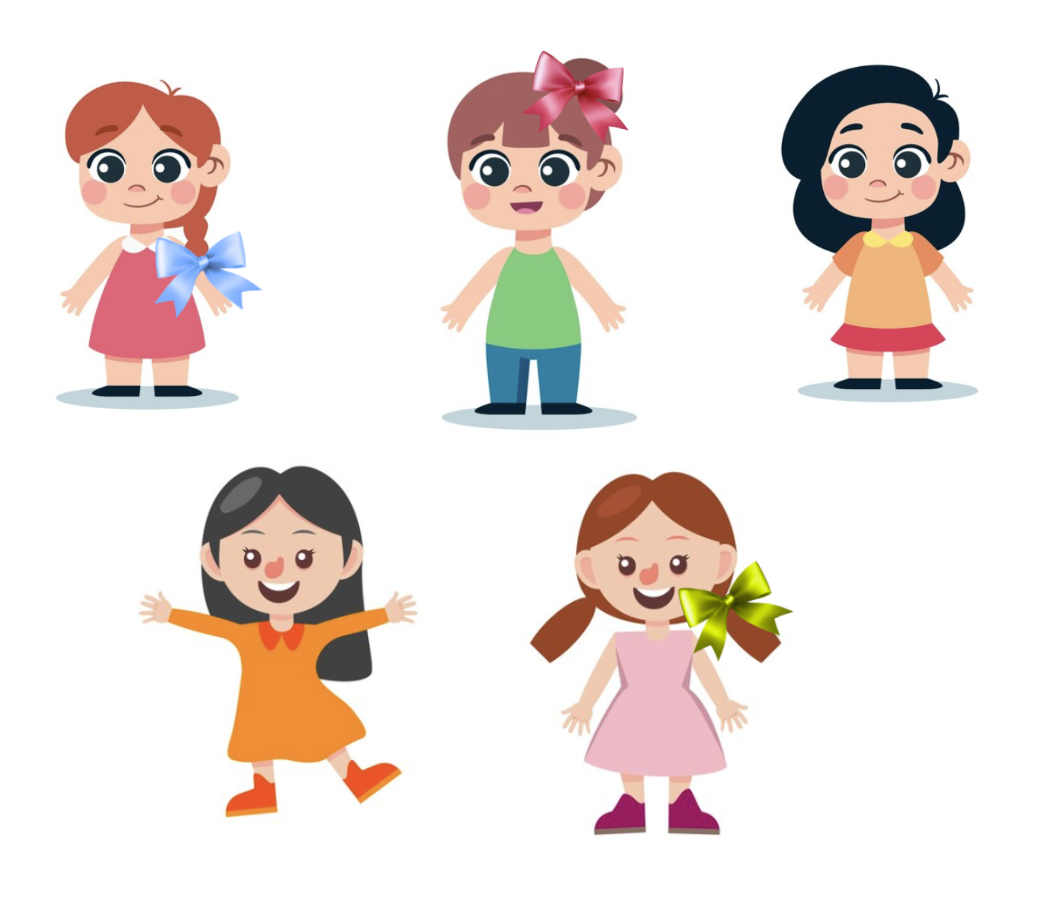
\includegraphics[width=\linewidth]{images/bows_0.png}
        \caption{$\le 1$}
    \end{minipage}\hfill
    \begin{minipage}{0.32\textwidth}
        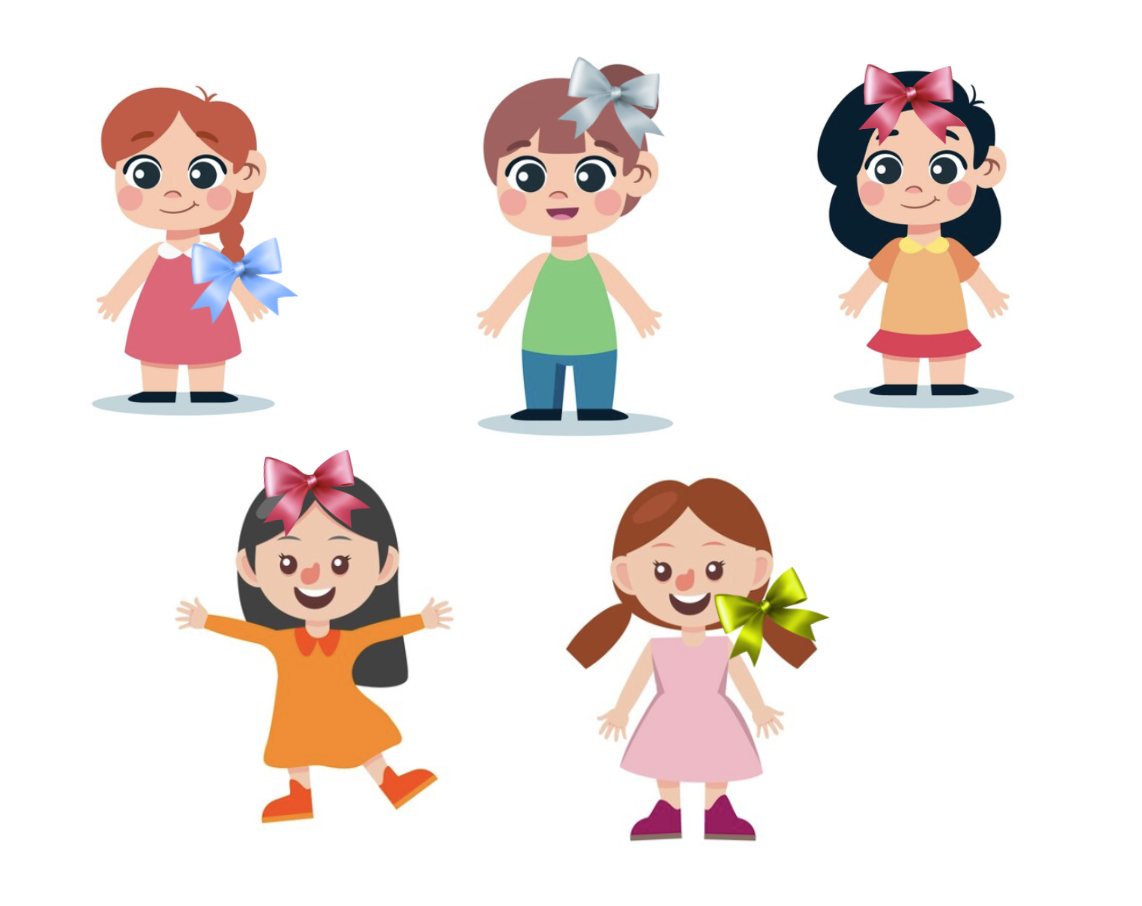
\includegraphics[width=\linewidth]{images/bows_1.png}
        \caption{$= 1$}
    \end{minipage}\hfill
    \begin{minipage}{0.32\textwidth}
        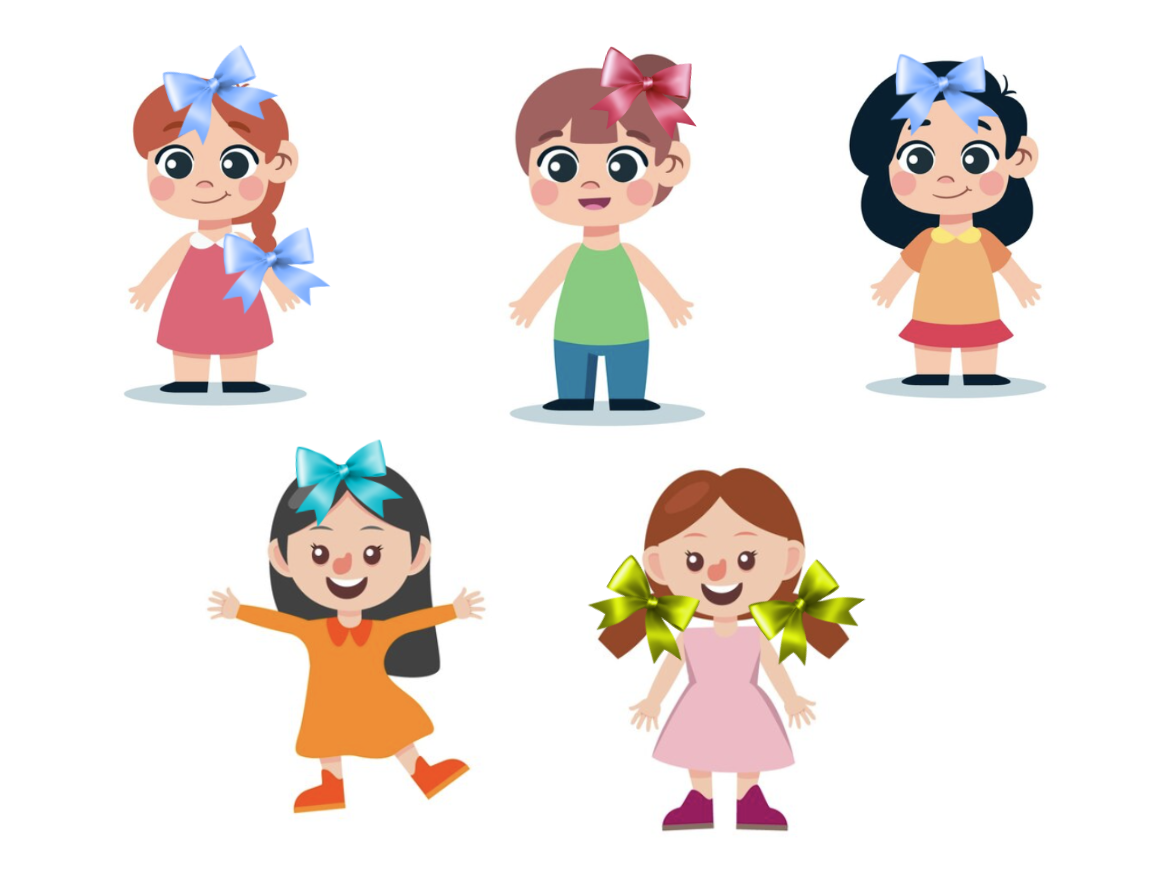
\includegraphics[width=\linewidth]{images/bows_2.png}
        \caption{$\ge 1$}
    \end{minipage}\hfill
\end{figure}

Стимул имел вид условного предложения. Протазис содержал именную группу в единственном числе и непереходный неаккузативный глагол, не являющийся глаголом появления. Стимулы были составлены таким образом, чтобы участник оценивал предложение дистрибутивно, то есть относительно каждой подситуации отдельно, а не всех ситуаций сразу.

Два варианта стимула — с порядком слов VS и SV — были даны в случайном порядке. Преамбула выполняла роль, схожую с ролью контекста, за исключением того что не была отражена на изображении. Преамбула вместе с двумя вариантами стимула выглядела как (\nextx).

\pex<stim>
    Каждая девочка в этой группе очень беспокоится о своей прическе.
    \begin{enumerate}
        \item Если бантик развязывается, девочка сразу идет к воспитателю.
        \item Если развязывается бантик, девочка сразу идет к воспитателю.
    \end{enumerate}
\xe

В зависимости от количества объектов в подситуациях удовлетворялись различные пресуппозиции определенных ИГ. В случаях с ровно одним объектом в каждой подситуации удовлетворялись и уникальность, и существование (такой вариант изображения служил бейзлайном). Изображения с одним и более объектом удовлетворяли пресуппозицию существования, но не уникальности; с одним или нулем — уникальности, но не существования.

Ожидалось, что в случае удовлетворения пресуппозициям (случай $=1$) именная группа должна, по правилу максимизации пресуппозиции, интерпретироваться как определенная и чаще находиться слева от глагола. При вариантах изображений $\le 1$ и $\ge 1$ более частотным выбором должны были быть предложения с порядком слов VS.

\subsection{Результаты и обсуждение}

В эксперименте приняло участие 42 человека. Результаты эксперимента представлены на графике ниже.

\begin{figure}
    \centering
    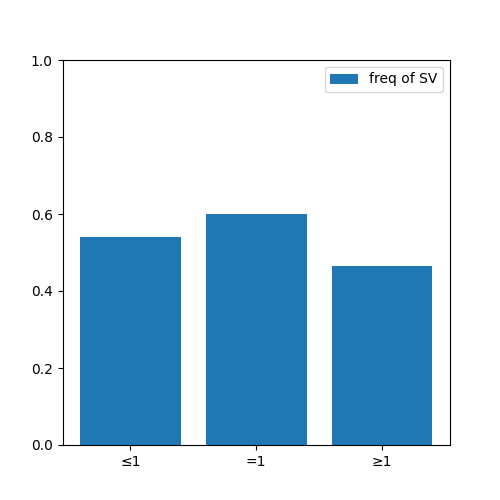
\includegraphics[width=0.6\textwidth]{images/plot.png}
    \caption{Зависимость частотности выбора SV от варианта стимула.}
    \label{plot}
\end{figure}

График изображает долю выбора порядка слов SV. В случае, когда все пресуппозиции удовлетворяются (столбец «$=1$»), SV действительно выбиралась чаще, чем в других ситуациях, что соответствует гипотезе. При этом различие слабее, чем ожидалось бы в случае полноценного нарушения пресуппозиции.

Для подтверждения гипотез был проведен статистический анализ с помощью модели линейной регрессии со смешанными эффектами, со случайными точками пересечения для участников и стимулов. Ниже описаны результаты анализа и обсуждаются теоретические следствия этих результатов.

\subsubsection{Уникальность}

Статистический анализ показал, что различие в частотности предглагольных субъектов при удовлетворении всех пресуппозиций и нарушении пресуппозиции уникальности статистически значимо ($z = 2.353, p = 0.019$). Это означает, что участники действительно выбирают порядок слов, основываясь на возможности уникально идентифицировать референт ИГ на каждой из подситуаций. Это подтверждает нашу гипотезу и демонстрирует, что эксперименты Шимика и Демиана не смогли выявить корреляцию по причинам иным, чем ее отсутствие.

Хотя сравнительный эксперимент для языков с артиклями проведен не был, можно обратить внимание на то, что корреляция достаточно слабая, несмотря на избавление от проблем дизайна предшествующих экспериментов. Можно было бы предположить, что значение уникальности является не пресуппозицией, а, например, отменяемой импликатурой. Однако импликатура уникальности референта едва ли является засвидетельствованной в языках мира, и еще более удивительна, если предположить, что природа определенности заключается в возможности идентификации референта \parencite[напр.][]{roberts2003uniquenessdefinitenoun}. Мы считаем, что такое объяснение маловероятно.

Мы считаем, что как минимум одной из причин низкой корреляции является дизайн стимулов. Если на одних из стимулов корреляция очень значительна, на других ее нет вовсе. Мы считаем, что более точно выверенные стимулы могут показать значительно большую корреляцию.

Несмотря на это, остается безусловным то, что порядок слов в русском языке позволяет значительно большую вариативность, чем европейские артикли. Возможно, причиной этого является наличие нескольких возможных дериваций, приводящих к одной и той же поверхностной реализации — SV, — некоторые из которых вводят пресуппозицию уникальности, а другие возможны контекстах, ограниченных другим образом. Альтернативным предположением может быть то, что пресуппозиция, вызванная порядком слов, имеет фундаментально иную природу — как, например, в теории \parencite{simik2021inherentvsaccidental}, — приводящую к другим возможностям аккомодации. Вероятно, релевантной является также связь порядка слов с информационной структурой.

\subsubsection{Существование}

Как можно увидеть из графика \ref{plot}, частотность выбора порядка SV в столбце «$\le1$» ближе к таковой в столбце «$=1$», чем в столбце «$\ge 1$». Действительно, статистический анализ показывает, что различие между столбцами «$\le1$» и «$=1$» незначимо (z = 1.152, p = 0.249). Это значит, что эксперимент не смог выявить влияние удовлетворения пресуппозиции существования на выбор порядка слов. Следовательно, вторая часть гипотезы не подтверждается.

Мы полагаем, что причина нечувствительности респондентов к пресуппозиции существования заключается в том, как оценивается истинность предложений в контексте множественных ситуаций. Когда в контексте имеется множество ситуаций, последующие предложения оцениваются только относительно ситуаций, для которых они релевантны. Ср. (\nextx).

\ex<>
    \{Петя каждый день ходит на работу мимо пекарни и иногда покупает там сосиску в тесте.\} Эту сосиску в тесте он съедает в обеденный перерыв.
\xe

В контексте (\lastx) вводится множество ситуаций — походов Пети на работу, — и в некоторых из этих ситуаций вводится новый референт — сосиска в тесте. Во втором предложении имеется именная группа с демонстративом, то есть требующая антецедента. Несмотря на то, что антецедент имеется не во всех ситуациях, введенных контекстом, предложение приемлемо, и его ассерция распространяется только на ситуации, где имеется сосиска в тесте. По-видимому, при интерпретации предложения имеющиеся в контексте ситуации, для которых предложение нерелевантно, отсеиваются.

Мы полагаем, что этот эффект имеет место и при оценке предложений в нашем эксперименте. Очевидно, если в вышеупомянутом примере девочка не имеет бантика, для нее протазис условного не может быть истиннен и, следовательно, условное нерелевантно. Эти ситуации игнорируются при оценке пресуппозиций предложения и, соответственно, пресуппозиция существования не нарушается.

Следует отметить, что то же самое не происходит с пресуппозицией уникальности, так как подситуации, в которых объекта более одного, все еще релевантны для интерпретации. Если девочка имеет более одного бантика, у нее все еще может развязаться бантик, и в наиболее естественном прочтении предложения в (\getfullref{stim}) ассертируют, что в таком случае она обратится к воспитателю. Исключить такие контекстные ситуации нельзя, и они влекут провал пресуппозиции.

\subsection{Заключение}

Исследование связи порядка слов и определенности представляет собой область, многократно исследованную, но по-прежнему имеющую множество неразрешенных вопросов в отношении как анализа, так и легитимности данных, на которые опираются теоретические исследователи. Экспериментальные исследования в этой области начались недавно и до сих пор не привели к успехам — корреляция порядка слов и определенности не была обнаружена.

Мы предложили дизайн эксперимента, решающий проблемы предыдущих исследований и способный выявить вышеупомянутую корреляцию. Поставленный нами эксперимент является пилотным — в дальнейшем планируеутся использовать этот дизайн с улучшенными стимулами и в эксперименте с большим количеством участников.

Было обнаружено, что по независимым причинам такой дизайн нечувствителен к пресуппозиции существования. Это ставит вопрос о том, как проверять пресуппозицию существования экспериментально вообще, если необходимо контролировать топикальность референта. Так или иначе, это выходит за рамки нашего исследования — мы заинтересованы в любой пресуппозиции, связанной с определенностью, и выявление влияния пресуппозиции уникальности для нас достаточно. 

Несмотря на то что форма стимулов создавалась так, чтобы возможно было проверить пресуппозицию существования, она оказалась достаточно эффективной для проверки пресуппозиции уникальности. Поэтому в дальнейшем этот дизайн планируется использовать для проверки только пресуппозиции максимальности. Необходимость обеспечивать возможность несоблюдения пресуппозиции существования значительно ограничивает множество подходящих стимулов, поэтому, избавившись от нее, мы получим доступ к более естественным контекстам и, следовательно, более качественным стимулам.

\printbibliography

\end{document}
